% Created 2021-04-14 Wed 15:57
% Intended LaTeX compiler: pdflatex
\documentclass[presentation,bigger,aspectratio=169]{beamer}
\usepackage[utf8]{inputenc}
\usepackage[T1]{fontenc}
\usepackage{graphicx}
\usepackage{grffile}
\usepackage{longtable}
\usepackage{wrapfig}
\usepackage{rotating}
\usepackage[normalem]{ulem}
\usepackage{amsmath}
\usepackage{textcomp}
\usepackage{amssymb}
\usepackage{capt-of}
\usepackage{hyperref}
\usepackage{xcolor}
\usepackage[]{minted}
\usepackage{tcolorbox}
\usepackage{etoolbox}\tcbuselibrary{magazine}
\BeforeBeginEnvironment{minted}{\begin{tcolorbox}[title=Input,colback=blue!5,colframe=blue!25!black,size=fbox, enforce breakable, break at=6cm]}%
\AfterEndEnvironment{minted}{\end{tcolorbox}}%
\BeforeBeginEnvironment{verbatim}{\begin{tcolorbox}[colback=white,size=fbox,enhanced jigsaw, enforce breakable,break at=6cm]}%
\AfterEndEnvironment{verbatim}{\end{tcolorbox}}%
\usepackage{inconsolata}
\usepackage[ngerman, germanb]{babel}
\usepackage [autostyle, english = american]{csquotes} \MakeOuterQuote{"}
\usepackage[utf8]{inputenc}\usepackage{tabulary,booktabs}\AtBeginEnvironment{tabulary}{\scriptsize}
\usepackage[fixlanguage]{babelbib}\selectbiblanguage{german}
\usepackage{csquotes,xpatch}\usepackage[natbib=true,style=apa,url=true,doi=true,annotation=false,eprint=false,backend=biber]{biblatex}\urlstyle{sf}
\DeclareLanguageMapping{austrian}{austrian-apa}
\DeclareSourcemap{\maps[datatype=bibtex]{\map{\step[fieldset=annotation,null]}}}\renewcommand*{\bibfont}{\scriptsize}
\addbibresource{~/Dropbox/org/ref/ref.bib}
%Global Background must be put in preamble
\usebackgroundtemplate%
{%
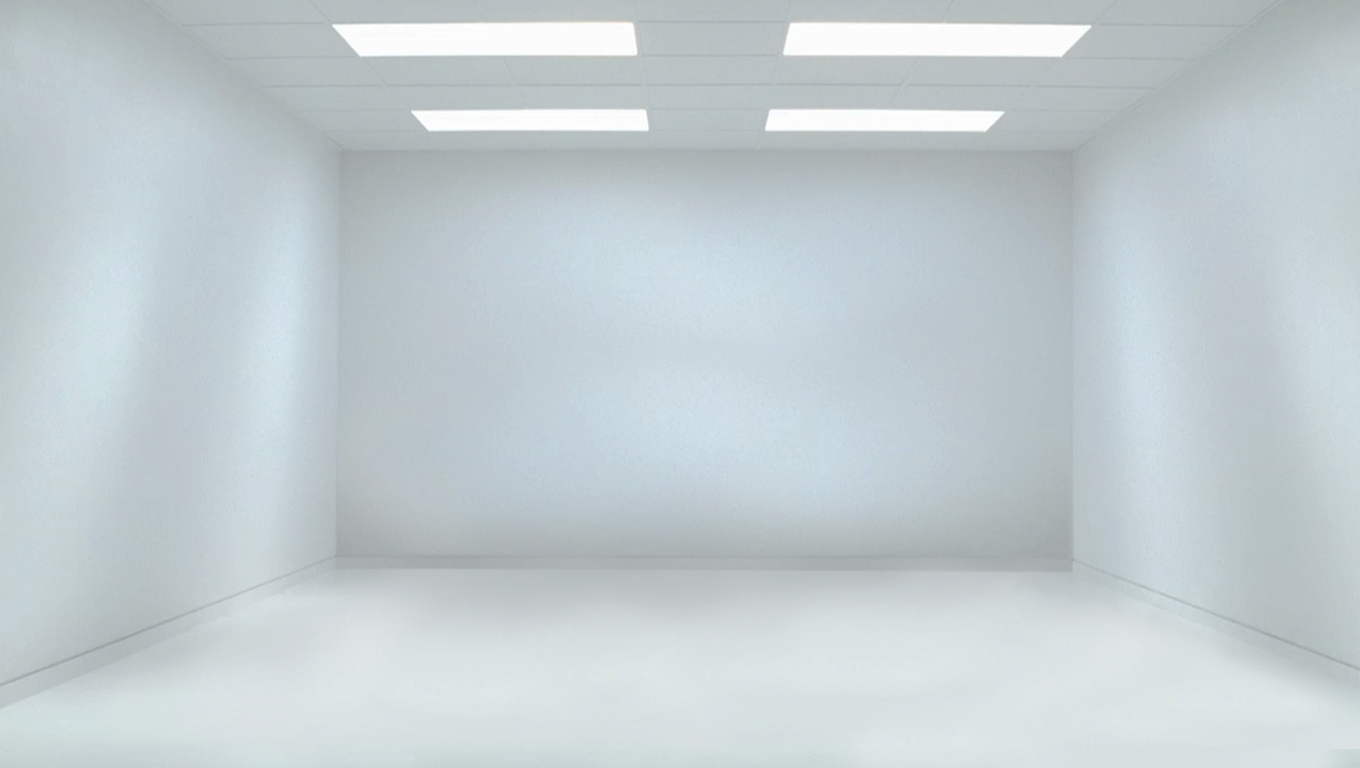
\includegraphics[width=1.175\paperwidth,height=1.05\paperheight]{./img/m1_praes_empty_10.jpg}%
}
\usetheme{default}
\author{user\thanks{user@mink}}
\date{15.4.2021}
\title{Interior Designer App: M1}
\subtitle{Problemanalyse}
\usetheme{Hannover}\usepackage{graphicx}\usepackage[overlay]{textpos}
\setbeamertemplate{bibliography item}{}
\setbeamertemplate{navigation symbols}{}
\definecolor{UBCblue}{HTML}{153a7a}\usecolortheme[named=UBCblue]{structure}
\usefonttheme{professionalfonts}
\setbeamerfont{note page}{family*=pplx,size=\footnotesize}
\definecolor{bgminted}{HTML}{eee9e9}
\definecolor{bluegray}{rgb}{0.54, 0.6, 0.8}
\definecolor{urlcolor}{HTML}{3399ff}
\definecolor{linkcolor}{HTML}{3399ff}
\definecolor{colorlinkscolor}{HTML}{3399ff}
\hypersetup{colorlinks=colorlinkscolor,linkcolor=linkcolor,urlcolor=urlcolor}
\setbeamertemplate{itemize items}[default]
\setbeamertemplate{enumerate items}[default]
\setbeamertemplate{items}[default]
\setbeamerfont*{title in sidebar}{shape=\scshape,size=\scriptsize}
\setbeamerfont*{author in sidebar}{family=\sfseries,size=\scriptsize}
\setbeamerfont*{section in sidebar}{family=\sfseries,size=\scriptsize}
\usetheme{Hannover}
\def\swidth{3.6cm}
\setbeamersize{sidebar width left=\swidth}
\setbeamertemplate{sidebar left}
{
{\usebeamerfont{title in sidebar}%
\vskip1.5em%
\usebeamercolor[fg]{title in sidebar}%
\insertshorttitle[width=\swidth,center,respectlinebreaks]\par%
\vskip1.25em%
}%
{%
\usebeamercolor[fg]{author in sidebar}%
\usebeamerfont{author in sidebar}%
\insertshortauthor[width=\swidth,center,respectlinebreaks]\par%
\vskip1.25em%
}%
\hbox to2cm{\hss\insertlogo\hss}
\vskip1.25em%
\hskip0.15cm\insertverticalnavigation{\swidth}%
\vfill
\hbox to2cm{\hskip0.25cm\usebeamerfont{subsection in
sidebar}\strut\usebeamercolor[fg]{subsection in
sidebar}\color{bluegray}\tiny\insertframenumber\hfill}%
\vskip6pt%
}%
\author[A.Oğuz, D.Pegler, S.Pum]{Asım Oğuz, Dominik Pegler, Sophia Pum}
\institute{Universität Wien, Fakultät für Informatik (SS2021)}
\hypersetup{
 pdfauthor={user},
 pdftitle={Interior Designer App: M1},
 pdfkeywords={},
 pdfsubject={},
 pdfcreator={Emacs 27.1 (Org mode 9.4.4)}, 
 pdflang={Germanb}}
\begin{document}

\maketitle

\section{Problembeschreibung}
\label{sec:orgf7cf806}

\begin{frame}[label={sec:org9e1a7f7}]{\vspace{2.2cm}\begin{center}\MakeUppercase{\insertsection}\end{center}}
\end{frame}

\begin{frame}[label={sec:org5a84d17}]{Interior Designer App}
\begin{block}{Problemstellung}
\begin{enumerate}
\item Welche Gestaltungsmöglichkeiten bieten Räume?
\item Wie können Möbel sinnvoll angeordnet werden?
\item Wie können auch Laien schnell zu Raumlösungen kommen und diese
visualisieren?
\end{enumerate}
\end{block}
\end{frame}
\begin{frame}[label={sec:org48c4964}]{Interior Designer App}
\begin{block}{Lösungsansatz: Mobile App}
\begin{itemize}
\item User fotografiert Raum
\item User wählt Möbelstück
\item App vermisst Raum, Möbelstück
\item User/App platziert Möbelstück im Raum
\end{itemize}
\vspace{0.8em}\hspace{2em}{\bfseries {\Longrightarrow} {\text{Augmented-Reality-Lösung (AR)}}}
\end{block}
\end{frame}

\begin{frame}[label={sec:org62f4709}]{Interior Designer App}
\begin{block}{Zusätzliches Feature: "Open Objects Sharing" (OOS)}
\begin{itemize}
\item 3D-Objekte können einfach erstellt und an andere Personen geschickt werden
\item Integration in Second-Hand-Apps wie Shpock oder Willhaben
\end{itemize}
\end{block}
\end{frame}

\section{Literaturrecherche}
\label{sec:org8a0c390}
\begin{frame}[label={sec:org6630e30}]{\vspace{2.2cm}\begin{center}\MakeUppercase{\insertsection}\end{center}}
\end{frame}

\begin{frame}[label={sec:orgc684750}]{Literatur}
\begin{block}{Schwerpunkt "Algorithmen und Augmented Reality"}
\begin{itemize}
\item \textcite{kanAutomatedInteriorDesign2017}
\item \textcite{sanduAugmentedRealityUses2018}
\item \textcite{moaresInterARInterior2020}
\end{itemize}
\end{block}
\end{frame}

\begin{frame}[label={sec:org1b5b5ae}]{Literatur I}
\begin{block}{Automated Interior Design}
\begin{itemize}
\item \textcite{kanAutomatedInteriorDesign2017}
\item Algorithmus:
\begin{itemize}
\item befüllt Räume selbstständig mit Einrichtung
\item folgt Interior Design Guidelines zu Funktion, Ästhetik \& Ergonomie
\item Schneidet gut ab in Wahrnehmungsstudie
\end{itemize}
\end{itemize}
\end{block}
\end{frame}

\begin{frame}[label={sec:org8fb3eef}]{Literatur II}
\begin{block}{Augmented Reality Uses in Interior Design}
\begin{itemize}
\item \textcite{sanduAugmentedRealityUses2018}
\item AR-unterstützte mobile Apps:
\begin{itemize}
\item OpenSource-Framework ArToolKit
\item Verbesserungsvorschläge zu aktuellen Implementierungen
\end{itemize}
\end{itemize}
\end{block}
\end{frame}

\begin{frame}[label={sec:org41f483b}]{Literatur III}
\begin{block}{Inter AR: Interior Decor App using Reality Technology}
\begin{itemize}
\item \textcite{moaresInterARInterior2020}
\item Arten von Augmented Reality
\begin{itemize}
\item marker-based vs. location-based vs. projection-based
\end{itemize}
\item Bericht Erstellung einer App mittels Google Cardboard SDK
\end{itemize}
\end{block}
\end{frame}

\begin{frame}[label={sec:org3e5f03a}]{Literatur}
\begin{block}{Takeaways}
\begin{itemize}
\item Wir bauen auf Bestehendem auf und erfinden nichts Neues
\item Wahl des AR-Frameworks miteinscheidend über den Funktionsumfang
\item Leere Räume
\item Potenzial ist da (siehe Wahrnehmungsstudie)
\end{itemize}
\end{block}
\end{frame}

\section{Konkurrenzanalyse}
\label{sec:org4aae12e}
\begin{frame}[label={sec:orgf91b76d}]{\vspace{2.2cm}\begin{center}\MakeUppercase{\insertsection}\end{center}}
\end{frame}

\begin{frame}[label={sec:orgeaf7846}]{Konkurrenzanalyse I}
\begin{block}{Houzz}
\begin{itemize}
\item \ldots{}
\item \ldots{}
\item \ldots{}
\end{itemize}
\end{block}
\end{frame}
\begin{frame}[label={sec:org4668e19}]{Konkurrenzanalyse II}
\begin{block}{Ikea Place}
\begin{itemize}
\item \ldots{}
\item \ldots{}
\item \ldots{}
\end{itemize}
\end{block}
\end{frame}
\begin{frame}[label={sec:org0f74d65}]{Konkurrenzanalyse III}
\begin{block}{Homestyler}
\begin{itemize}
\item \ldots{}
\item \ldots{}
\item \ldots{}
\end{itemize}
\end{block}
\end{frame}
\section{Nutzeranalyse}
\label{sec:org2a16f16}
\begin{frame}[label={sec:org92db75e}]{\vspace{2.2cm}\begin{center}\MakeUppercase{\insertsection}\end{center}}
\end{frame}

\begin{frame}[label={sec:org793c28d}]{Nutzeranalyse I}
\begin{block}{Aufgaben der Nutzer}
\begin{itemize}
\item Schnelles Skizzieren von Innenarchitekturen
\item Schnelles Visualisieren
\item Anderen Personen vorführen
\end{itemize}
\end{block}
\end{frame}

\begin{frame}[label={sec:orge41dd1f}]{Nutzeranalyse II}
\begin{block}{Ziele der Nutzer}
\begin{itemize}
\item Zeit- und Kostenersparnis (keine Beratung nötig)
\item Konkretere Vorstellungen zu entwickeln
\item Bessere und nachhaltigere Entscheidungen treffen
\end{itemize}
\end{block}
\end{frame}

\begin{frame}[label={sec:org5a17150}]{Nutzeranalyse III}
\begin{block}{Potenzielle Probleme mit dem System}
\begin{itemize}
\item User fühlen sich von App nicht angesprochen
\item Kein Zusatznutzen zu bereits vorhandenen Tools
\item Funktionalitäten zu eingeschränkt (nur bestimmte Möbel/Objekte,
Limit bei Anzahl)
\item Aufbau und Logik des Programms zu kompliziert
\item Zu lange Ladezeiten (bei mobilen Apps besonders wichtig!)
\item Freezing oder Absturz der App
\item Läuft nicht auf allen Smartphones
\end{itemize}
\end{block}
\end{frame}

\section{Personas}
\label{sec:org9e8dc25}
\begin{frame}[label={sec:org775fb9f}]{\vspace{2.2cm}\begin{center}\MakeUppercase{\insertsection}\end{center}}
\begin{center}
\vskip -12.5em 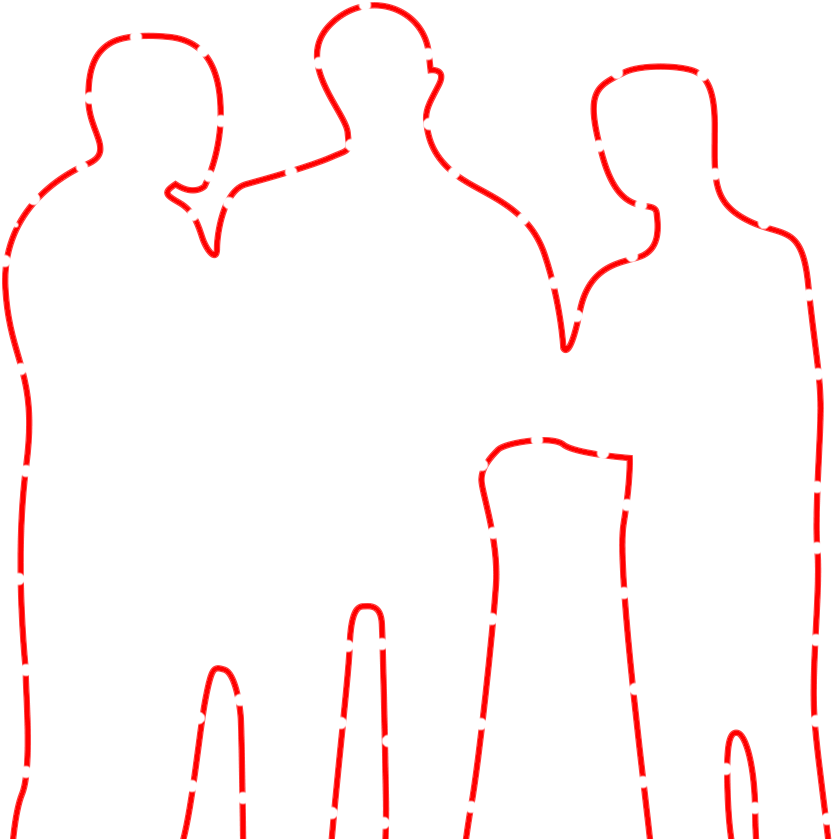
\includegraphics[height=140px]{./img/m1_praes_ol_persona3.png}
\end{center}
\end{frame}
\begin{frame}[label={sec:org568c2f9}]{Personas I}
\begin{block}{Primäre Persona 1: Tobias Ebner}
\begin{center}

\includegraphics[width=90px]{./img/m1_persona_1_idealist.png}
\end{center}
\begin{itemize}
\item Typ: Idealist
\item Alter: 25
\item Beruf: Grafikdesigner
\end{itemize}
\end{block}
\end{frame}
\begin{frame}[label={sec:org70c97a1}]{Personas II}
\begin{block}{Primäre Persona 2: Carina Winkler}
\begin{center}
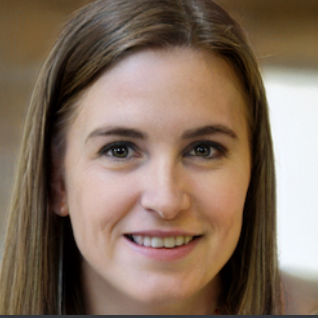
\includegraphics[width=90px]{./img/m1_persona_2_rational.png}
\end{center}
\begin{itemize}
\item Typ: Rational
\item Alter: 32
\item Beruf: Ärztin
\end{itemize}
\end{block}
\end{frame}
\begin{frame}[label={sec:orgbf423b8}]{Personas III}
\begin{block}{Sekundäre Persona: Felix Schuster}
\begin{center}
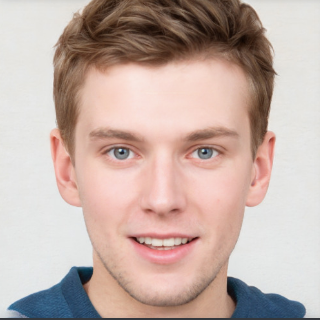
\includegraphics[width=90px]{./img/m1_persona_3_rational.png}
\end{center}
\begin{itemize}
\item Typ: Minimalist
\item Alter: 20
\item Beruf: Student
\end{itemize}
\end{block}
\end{frame}
\begin{frame}[label={sec:orgf436b61}]{Personas IV}
\begin{block}{Negative Persona: Sabine Gruber}
\begin{center}
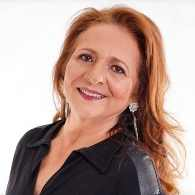
\includegraphics[width=90px]{./img/m1_persona_4_guardian.jpg}
\end{center}
\begin{itemize}
\item Typ: Guardian
\item Alter: 64
\item Beruf: Verkäuferin
\end{itemize}
\end{block}
\end{frame}
\section{Aufgabenanalyse}
\label{sec:org747a778}
\begin{frame}[label={sec:orgdad479b}]{\vspace{2.2cm}\begin{center}\MakeUppercase{\insertsection}\end{center}}
\end{frame}
\begin{frame}[label={sec:org11090eb}]{Aufgabenanalyse}
\begin{center}
\begin{tabular}{lcc}
\toprule
\(\downarrow\) Task / User \(\to\) & Carina Winkler & Tobias Ebner\\
\midrule
App downloaden & + & +\\
Raum fotografieren & + & +\\
Möbel scannen & \textasciitilde{} & \textasciitilde{}\\
Vorhandene Möbel auswählen & + & +\\
Raum gestalten & \textasciitilde{} & \textasciitilde{}\\
Design abspeichern & + & +\\
\bottomrule
\end{tabular}
\end{center}
\end{frame}

\section{Projektmanagement}
\label{sec:org52664e1}
\begin{frame}[label={sec:org95d7c5f}]{\vspace{2.2cm}\begin{center}\MakeUppercase{\insertsection}\end{center}}
\end{frame}

\begin{frame}[label={sec:orgc2a7d0a}]{Projektmanagement I}
\begin{block}{Abstimmung und Planung}
\begin{itemize}
\item Simple Github-Page mit
\begin{itemize}
\item TODOs
\item Terminen und Deadlines
\item Zuordnung der Aufgaben
\item Notizen
\item Updates zum Fortschritt
\end{itemize}
\end{itemize}
\end{block}
\end{frame}

\begin{frame}[label={sec:orge8c7800}]{Projektmanagement II}
\begin{block}{Aufgabenverteilung}
\begin{itemize}
\item nach Interesse und Themenblöcken
\item kurzfristig
\item flexibel
\end{itemize}
\end{block}
\end{frame}
\begin{frame}[label={sec:org9358352}]{Projektmanagement III}
\begin{block}{Ziele des Projekts}
\begin{itemize}
\item Prototyp einer App entwickeln, die so simpel wie möglich ist
\item Zumindest Teile des Projekts später in Realität umsetzen
\item Neue Technologie kennenlernen
\end{itemize}
\end{block}
\end{frame}
\begin{frame}[label={sec:org18b900f}]{Projektmanagement IV}
\begin{block}{Nicht-Ziele des Projekts}
\begin{itemize}
\item Bestehendes wiederholen
\item Nice-To-Have-Features ohne relevanten Zusatznutzen implementieren (z.B. weil
die Technik dahinter spannend ist) \(\to\) alles weglassen, das nicht mit
den Nutzerzielen zu tun hat
\end{itemize}
\end{block}
\end{frame}

\section*{Literatur}
\label{sec:orgf99fea0}
\begin{frame}[allowframebreaks]{Literatur}
\printbibliography[heading=none]
\end{frame}
\appendix
\end{document}
